% This must be in the first 5 lines to tell arXiv to use pdfLaTeX, which is strongly recommended.
\pdfoutput=1
% In particular, the hyperref package requires pdfLaTeX in order to break URLs across lines.

\documentclass[11pt]{article}

% Change "review" to "final" to generate the final (sometimes called camera-ready) version.
% Change to "preprint" to generate a non-anonymous version with page numbers.
\usepackage[final]{acl}

% Standard package includes
\usepackage{times}
\usepackage{latexsym}

\usepackage{hyperref}
\usepackage{cleveref}
\usepackage{makecell}
\usepackage{array}

\usepackage{rotating}
\usepackage{array,multirow,graphicx}



% For proper rendering and hyphenation of words containing Latin characters (including in bib files)
\usepackage[T1]{fontenc}
% For Vietnamese characters
% \usepackage[T5]{fontenc}
% See https://www.latex-project.org/help/documentation/encguide.pdf for other character sets

% This assumes your files are encoded as UTF8
\usepackage[utf8]{inputenc}

% This is not strictly necessary, and may be commented out,
% but it will improve the layout of the manuscript,
% and will typically save some space.
\usepackage{microtype}

% This is also not strictly necessary, and may be commented out.
% However, it will improve the aesthetics of text in
% the typewriter font.
\usepackage{inconsolata}

%Including images in your LaTeX document requires adding
%additional package(s)
\usepackage{graphicx}

\usepackage{tikz}
% \def\checkmark{\tikz\fill[scale=0.4](0,.35) -- (.25,0) -- (1,.7) -- (.25,.15) -- cycle;}
\newcommand{\tikzxmark}{%
\tikz[scale=0.23] {
    \draw[line width=0.7,line cap=round] (0,0) to [bend left=6] (1,1);
    \draw[line width=0.7,line cap=round] (0.2,0.95) to [bend right=3] (0.8,0.05);
}}
\newcommand{\tikzcmark}{%
\tikz[scale=0.23] {
    \draw[line width=0.7,line cap=round] (0.25,0) to [bend left=10] (1,1);
    \draw[line width=0.8,line cap=round] (0,0.35) to [bend right=1] (0.23,0);
}}

\usetikzlibrary{positioning, shapes.multipart}
\newcommand{\voc}[1]{\texttt{#1}}

\newcommand{\ensuretext}[1]{#1}
\newcommand{\nertcomment}[4]{\ensuretext{\textcolor{#3}{[\ensuretext{\textcolor{#3}{\ensuremath{^{\textsc{#1}}_{\textsc{#2}}}}} #4]}}}
\newcommand{\sw}[1]{\nertcomment{S}{W}{orange}{#1}}
\newcommand{\ejm}[1]{\nertcomment{E}{M}{blue}{#1}}
\newcommand{\ri}[1]{\nertcomment{R}{I}{purple}{#1}}

% If the title and author information does not fit in the area allocated, uncomment the following
%
%\setlength\titlebox{<dim>}
%
% and set <dim> to something 5cm or larger.

\title{Generating Text from Uniform Meaning Representation}

% Author information can be set in various styles:
% For several authors from the same institution:
% \author{Author 1 \and ... \and Author n \\
%         Address line \\ ... \\ Address line}
% if the names do not fit well on one line use
%         Author 1 \\ {\bf Author 2} \\ ... \\ {\bf Author n} \\
% For authors from different institutions:
% \author{Author 1 \\ Address line \\  ... \\ Address line
%         \And  ... \And
%         Author n \\ Address line \\ ... \\ Address line}
% To start a separate ``row'' of authors use \AND, as in
% \author{Author 1 \\ Address line \\  ... \\ Address line
%         \AND
%         Author 2 \\ Address line \\ ... \\ Address line \And
%         Author 3 \\ Address line \\ ... \\ Address line}

\author{Emma Markle \\
  Amherst College \\
  \texttt{emarkle26@amherst.edu} \\\And
  Reihaneh Iranmanesh \\
  Amherst College \\
  \texttt{riranmanesh25@amherst.edu} \\\And
  Shira Wein \\
  Amherst College \\
  \texttt{swein@amherst.edu} \\}


\begin{document}
\maketitle
\begin{abstract}
Uniform Meaning Representation (UMR) is a recently developed graph-based semantic representation, which expands on Abstract Meaning Representation (AMR) in a number of ways, in particular through the inclusion of document-level information and multilingual flexibility. In order to effectively adopt and leverage UMR for downstream tasks, efforts must be placed toward developing a UMR technological ecosystem.
Though still limited amounts of UMR annotations have been produced to date, in this work, we investigate the first approaches to producing text from multilingual UMR graphs: (1)~a pipeline conversion of UMR to AMR, then using AMR-to-text generation models, (2)~fine-tuning large language models with UMR data, and (3)~fine-tuning existing AMR-to-text generation models with UMR data.
% fine-tune an existing AMR-to-text generation model with UMR data.
Our best performing model achieves an multilingual BERTscore of 0.825 for English and 0.882 for Chinese when compared to the reference, which is a promising indication of the effectiveness of fine-tuning approaches for UMR-to-text generation with even limited amounts of UMR data.\footnote{Our checkpoints and code are available at \url{https://github.com/ACNLPlab/UMR-Text-Gen}{}}
% \footnote{Our checkpoints and code will be released upon publication.}
\end{abstract}

\section{Introduction}

\begin{figure}[t]
    % \small
% \begin{subfigure}
\centering
%\includegraphics[trim={0cm 1cm 0cm 0cm},clip, scale=0.4]{Unknown.png}
\resizebox{\linewidth}{!}{
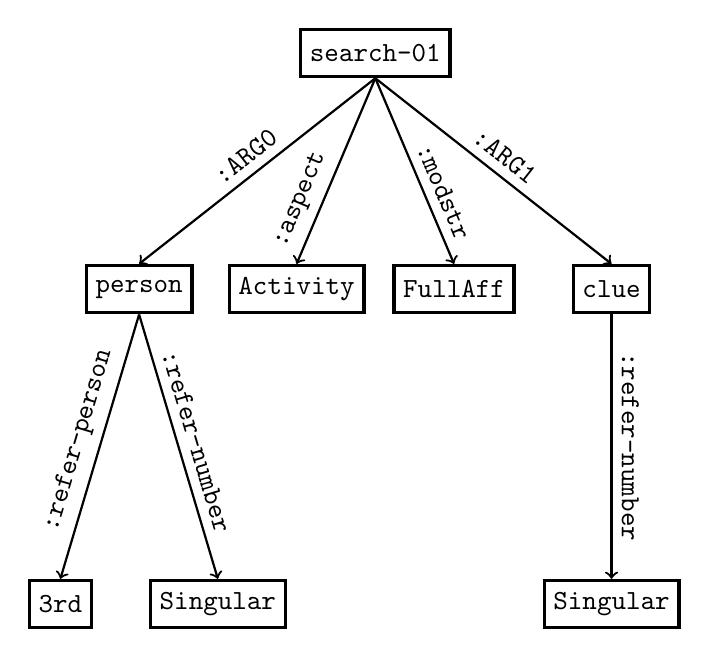
\begin{tikzpicture}[
blue/.style={rectangle, draw=black, very thick, minimum size=6mm},
]
	% Nodes
	\node[blue](s) at (10,10) {\voc{search-01}};
	\node[blue](p) at (7,7) {\voc{person}};
    \node[blue](t) at (6,3) {\voc{3rd}};
    \node[blue](sing1) at (8,3) {\voc{Singular}};
	\node[blue](a) at (9,7) {\voc{Activity}};
	\node[blue](f) at (11,7) {\voc{FullAff}};
    \node[blue](c) at (13,7) {\voc{clue}};
    \node[blue](sing2) at (13,3) {\voc{Singular}};
	% Edges
	\draw[->, thick] (s.south) -- (p.north) node[midway, above, sloped] {\voc{:ARG0}};
	\draw[->, thick] (s.south) -- (c.north) node[midway, above, sloped] {\voc{:ARG1}};
 	\draw[->, thick] (s.south) -- (a.north) node[pos=0.7, sloped, above] {\voc{:aspect}};
 	\draw[->, thick] (s.south) -- (f.north) node[pos=0.65, sloped, above] {\voc{:modstr}};
    \draw[->, thick] (c.south) -- (sing2.north) node[midway, above, sloped] {\voc{:refer-number}};
    \draw[->, thick] (p.south) -- (sing1.north) node[midway, above, sloped] {\voc{:refer-number}};
    \draw[->, thick] (p.south) -- (t.north) node[midway, above, sloped] {\voc{:refer-person}};

    
\end{tikzpicture}}
% \end{subfigure}
% \begin{subfigure}
\smallbreak
\small
\begin{verbatim}
(s / search-01
  :Arg0 (p / person
    :refer-person 3rd
    :refer-number Singular)
  :Arg1 (c / clue
    :refer-number Singular)
  :aspect Activity
  :modstr FullAff)
\end{verbatim}
% \end{subfigure}
\caption{UMR graph for the sentence ``He was searching for a clue'' in graph form (top) and in `PENMAN' notation \citep{kasper-1989-flexible} (bottom).
% Note that 3rd and Singular are not concepts but attributes.
}
\label{fig:umr_example}
\end{figure}

Uniform Meaning Representation (UMR) is a graph-based semantic representation designed to capture the core elements of meaning for a wide range of languages \citep{van2021designing}.

The UMR project has seen recent progress but is still in the early stages, with new resources such as an online web annotation tool \citep{ge-etal-2023-umr} and a relatively small recently-released annotated dataset \citep{bonn-etal-2024-building-broad}.


Abstract Meaning Representation \citep[AMR;][]{banarescu-etal-2013-abstract}
on which UMR is based, has seen success and adoption by the broader NLP community, and this is in large part due to the substantial efforts made towards high-quality text-to-AMR parsing and AMR-to-text generation models \citep{sadeddine-etal-2024-survey}.
\footnote{The breadth of parsing and generation work for AMR is shown in the \href{https://nert-nlp.github.io/AMR-Bibliography/}{AMR Bibliography}.}
This progress on parsing and generation is integral to being able to incorporate AMR graphs into downstream applications and studies of language \citep{wein-opitz-2024-survey}. Thus, in order to see similar success for UMR, efforts towards UMR-to-text generation and text-to-UMR parsing are critical.

In this work, we leverage the recent release of human-annotated UMR data (detailed in \Cref{ssec:data})
to tackle UMR-to-text generation and introduce the first UMR-to-text generation models. We investigate generation from the six languages included in the UMR v1.0 dataset: English, Chinese, Sanapaná, Arápaho, Kukama, and Navajo.
% We develop three distinct approaches to UMR-to-text generation, which utilize existing AMR-to-text generation methodologies to different degrees. 
% Specifically, we develop models by: (1)~a pipeline approach converting UMR to AMR then using AMR-to-text generation models, (2)~fine-tuning large language models with UMR data, and (3)~fine-tuning existing AMR-to-text generation models with UMR data. Additionally, we collect baseline results by passing in UMR graphs as-is straight into AMR-to-text generations.
% \sw{shira to do: Contributions}
Our approaches and contributions include:
\begin{itemize}
\addtolength\itemsep{-3mm}
    \item A baseline analysis as to how well six AMR-to-text generation models generate text from UMR out-of-the-box (\Cref{sec:baseline}).
    % \ri{A baseline analysis as to how well six AMR-to-text generation models generate **text** from UMR.}
    \item A novel pipelined approach to UMR-to-text generation, which converts UMR graphs into AMRs, then uses them as input to AMR-to-text generation models (\Cref{sec:conversion}).
    \item 
    % \sw{split into two bullet points via new section 7 fine-tuned llms}
    Seven fine-tuned UMR-to-text generation models, three using pretrained large language models and four pretrained AMR-to-text generation models as bases, demonstrating the potential benefits of leveraging AMR graphs for UMR tools (\Cref{sec:fine-tuned}). 
    % \item Thorough human evaluations for English and Chinese with respect to generated text fluency and adequacy, as well as automatic metric evaluations for all six languages, resulting in a model ranking and assertion of our best-performing model (\Cref{ssec:evaluation}).
\end{itemize}
% \sw{shira to do: specific details of experimentation here and models introduced, including the baseline and the three models}


\section{Uniform Meaning Representation}

UMR is based on Abstract Meaning Representation (AMR), which was designed for English 
\citep{banarescu-etal-2013-abstract} but has since seen various cross-lingual extensions and applications \citep{10.1162/coli_a_00503}. 
% \ejm{this is the third time we say UMR is based on AMR, is this too much?} \sw{where are the other two times?}

Similarly to AMR, UMR annotations are rooted, directed graphs that capture the meaning of a sentence \citep{van2021designing}.
% UMR includes both sentence and document-level graphs. At the document-level, UMR annotations include coreferential, temporal, and modal relations for the entire document. 
UMR incorporates aspect and modality at the sentence-level and additionally includes document-level graphs, enabling annotation of coreferential relations.
Alignments between the coreferential elements are also provided.
% \ejm{add something here for alignment}

In order to ensure that UMR could reflect meaning for many languages, the UMR schema is flexible in its annotation while ensuring consistency across languages.
At the sentence-level, UMR accounts for linguistic diversity across languages through the use of a lattice-like annotation schema \citep{van-gysel-etal-2019-cross}. This enables annotators to choose a more coarse-grained versus a more fine-grained annotation for numerous annotation categories (including discourse relations, modality, number, spatial relations, aspect, and temporality) based on the features of the language being annotated.
Particular care is also given to the annotation of low- or no-resource languages \citep{vigus-etal-2020-cross}, as ``Stage 0'' annotation is performed for languages that do not have existing rolesets available. Stage 0 annotation enables annotators to establish predicate-argument structures and develop rolesets while performing UMR annotation.
% UMR also includes information about aspect, modality, and scope at the sentence-level.

UMR successfully accommodates the multilingual issues addressed in individual language adaptations of AMR, showing its promise as a multilingual representation \citep{wein-bonn-2023-comparing}. Its effectiveness at capturing meaning across languages was also indicated in the pilot annotation of UMR in four indigenous languages \citep{van-gysel-etal-2021-theoretical}.

\Citet{chun-xue-2024-pipeline} released a text-to-UMR parser, which produces the document-level UMR graph based on the contents of the sentence, and the sentence-level UMR graph by running existing text-to-AMR parsers and then converting the AMR into a UMR.\footnote{This pipelined parsing approach mirrors our baseline approach, in the reverse direction.}

Recent work has investigated
automated Arápaho UMR annotation \citep{buchholz-etal-2024-bootstrapping-umr}, automatic annotation of tense and aspect for UMR \citep{chen-etal-2021-autoaspect}, and conversion of AMR graphs to UMR \citep{bonn-etal-2023-mapping,post-etal-2024-accelerating}.
Special attention has been given to UMR annotation of multi-word expressions \citep{bonn-etal-2023-umr} and Chinese verb compounds \citep{sun-etal-2023-umr}.

\section{Methodology}
% We started by splitting the UMR data  into training, dev, and test sets. Then, for our baseline approach (\Cref{sec:baseline}), we ran AMR-to-text generators on the UMR data to see how well the text came out with no prior training on UMR data, comparing the results to the reference sentences.
We develop four approaches, including our baseline, and evaluate them on the UMR data \citep{bonn-etal-2024-building-broad}, which we divide into train, dev, and test splits.

Our baseline approach uses six AMR-to-text generation models, passing the sentence-level UMR graphs as input.
Next, using the same six models used for our baseline, we developed a pipeline approach (\Cref{sec:conversion}) to UMR-to-text generation, which involved first converting the UMR graphs to AMR graphs, and then passing the converted AMR graphs as input to the models. 
Then, based on the baseline performance of the AMR-to-text generation models, we fine-tuned the top performing models as well as three large language models (with no AMR input) on the UMR training set (\Cref{sec:fine-tuned}).
% \sw{add sentence here about section 7 fine-tuned LLMs}


\subsection{Data}
\label{ssec:data}
We used the first release of UMR data \citep{bonn-etal-2024-building-broad}, which contains annotations in six languages: English, Chinese, and four languages indigenous to the Americas: Arápaho, Navajo, Sanapaná, and Kukama. 
The English data contains
LORELEI news text and a description of a silent film. The Chinese data consists of wikinews sentences.
Arápaho, Navajo, and Kukama annotations all represent narrative documents, while it is not clear what genre the Sanapaná annotations are \citep{bonn-etal-2024-building-broad}.
We first took out the English UMR data that contains equivalent AMRs in the AMR3.0 dataset \citep{knight_amr_3.0}, as to avoid leakage and unfair evaluations of models which contain the corresponding AMR data. This consisted of 66 English UMRs.
Then, we divided it into training and testing sets.


Not all annotations contained sentence-level and document-level graphs.
% however, the split of the data remains the same. \ejm{this disagrees with table 1, the splits are different as we only count doc and having doc level graph and alignment. we still used same number as sentence data but only the number in parentheses actually had doc data}
This is because some annotations without document-level data contained alignment data or could be referenced in other document-level annotations.
% The final amount of graph data we had for each language is as follows:
% \begin{itemize}
% \addtolength\itemsep{-3mm}
%     \item English: 143 sent-level graphs, 136 doc-level
%     \item Chinese: 358 sent-level graphs, 358 doc-level
%     \item Arápaho: 406 sent-level graphs, 109 doc-level
%     \item Navajo: 506 sent-level graphs, 168 doc-level
%     \item Sanapaná: 602 sent-level graphs, 602 doc-level
%     \item Kukama: 105 sent-level graphs, 86 doc-level
% \end{itemize}
Our final data split was 70\% for training, 10\% for dev, and 20\% for testing (the number of sentences for each language is shown in \Cref{tab:split}). 

\begin{table}
    \hspace{-1cm}
    \small
    \begin{center} 
    \begin{tabular}{|c|c|c|c|}
    \hline
    Language&Training (70\%)&Dev (10\%)&Test (20\%)\\
    \hline
    English& 100 (96)& 13 (13)& 30 (28)\\ 
    \hline
    Chinese& 236 (236)& 40 (40)& 82 (82)\\
    \hline
    Arápaho& 256 (46)& 36 (7)& 114 (54)\\
    \hline
    Navajo& 371 (148)& 52 (20)& 83 (0)\\
    \hline
    Sanapaná& 433 (366)& 62 (53)& 107 (104)\\
    \hline
    Kukama& 76 (76)& 10 (10)& 19 (0)\\
    \hline
    Total&  1472 (968)& 213 (143)& 435 (268)\\
    \hline
    \end{tabular}
    \end{center}
    \caption{Our training, dev, and test splits for the UMR data at the sentence-level, with the amount of sentence-level annotations that also had document-level information displayed in parentheses. We only counted data as being document-level if it contained both alignment and a document-level graph that was more complex than \texttt{(s / sentence)}.}
    \label{tab:split}
\end{table}


\subsection{Automatic Evaluation}
\label{ssec:evaluation}
We evaluated the generated text via both automatic metrics as well as human evaluation.

We compare the generated text from each of our approaches against the references (the ground-truth sentences that were annotated) by using BERTscore \citep{zhang2019bertscore}, given its previously evidenced correlation with human judgments for AMR-to-English text generation \citep{manning-etal-2020-human}. Specifically, we compare sentence similarity using multilingual BERTscore. We also use METEOR \citep{banerjee-lavie-2005-meteor} and BLEU \citep{papineni2002bleu} to enable ease of comparison with future work.

\subsection{Indigenous Language Evaluation}
During initial experimentation, we saw primarily positive quantitative indications as far as the ability of our models to produce text in the four indigenous languages, 
%\ejm{please re-write the following sentence for clarity and also include the amrlib scores since we reference them in the next paragraph}
for example, multilingual BERTscores of 0.799 for Navajo, 0.816 for Sanapaná, 0.780 for Arápaho, and 0.673 for Kukama, as generated by amrlib trained on all languages' sentence-level data.
%\ejm{@emma please provide some examples of the scores we were seeing for these languages for the best models. thanks!}.

However, given the fact that these languages are extremely low-resource and are not likely to be well-evaluated by BERTscore, METEOR, and BLEU, 
we consulted with speakers of Arápaho and Navajo to provide a human evaluation of the generated text.
We provided the output from the amrlib sentence-level model fine-tuned on all languages, as the quantitative indications of the text quality were positive. Our Arápaho and Navajo speakers indicated that, while
% - \sw{shira to do: check which data they reviewed} sentence-level amrlib fine-tuned (on all languages)
these fine-tuned models did do a fairly good job at imitating the script of the four indigenous languages, the output nonetheless was nonsensical and ungrammatical. As such, we opted against a full human evaluation for the four indigenous languages, with the understanding that even our top-performing models were outputting gibberish for these languages. This is likely because these four languages are all extremely low-resource and exhibit morphological complexity that would require additional resources for coherent text generation.
% the amrlib fine-tuned model still struggled however to produce chinese characters

As a result, we moved forward with evaluating our approaches and models exclusively in English and Chinese (both with regard to automatic evaluation and human evaluation). We still leveraged the indigenous language data in the UMR splits (as indicated in \Cref{tab:split}) for our model fine-tuning (\Cref{sec:fine-tuned}).

\subsection{Human Evaluation}
In order to validate the quantitative results obtained by the automatic metrics, we perform a human evaluation. Six college students participated in the evaluation of the English and Chinese texts, who were native speakers of English and Chinese accordingly.
Each annotator judged fluency and adequacy on a scale from 1-4. Fluency was judged first, without exposure to the reference, and then adequacy was judged in relation to the reference.

There were a total of four surveys: English fluency, English adequacy, Chinese fluency, and Chinese adequacy, each of which contained 25 questions. For English, we chose to exclude the 5 shortest sentences, which left us with a final set of 25 sentences. For Chinese, we randomly selected the sentences.
%\ejm{add here how we picked the sentences. random 25 for chinese, hand-selected for english}
Each question in the English fluency and adequacy surveys displayed six sentences, with five being from each of our top-performing models from each approach (with two models included for some approaches), as well as the reference.
% \ejm{this is not correct, only 5 sentences were from top models, one was a reference}
% \begin{itemize}
% \addtolength\itemsep{-3mm}
%     \item Reference sentence
%     \item UMR-to-AMR conversion graph generated to text via BiBL
%     \item BiBL sentence-level fine-tuned on English data only
%     \item baseline BiBL generated text
%     \item SPRING document-level fine-tuned on English data only
%     \item mBART sentence-level fine-tuned on all language data
% \end{itemize}
% The Chinese fluency and Chinese adequacy surveys displayed six sentences, one sentence for each of these categories:
% \begin{itemize}
% \addtolength\itemsep{-3mm}
%     \item Reference sentence
%     \item UMR-to-AMR conversion graph generated to text via Smelting
%     \item BiBL sentence-level fine-tuned on Chinese data only
%     \item Baseline Smelting generated text
%     \item SPRING document-level fine-tuned on Chinese data only 
%     \item mT5 sentence-level fine-tuned on all language data
% \end{itemize}
% It is important to note that both fluency surveys randomized the order of all six sentences, while the adequacy surveys displayed the reference sentence at the top and then randomized the other five models' outputs.
The instructions provided to the human raters for the English fluency and adequacy surveys can be seen in \Cref{fig:fluency_instructions,fig:adequacy_instructions}.\footnote{The Chinese instructions are identical to the English instructions but include the word ``Chinese'' instead of ``English.''}

% \sw{images of the survey here, description of the survey} 
% \ejm{images of survey below, description of survey above. thanks! :)}
\begin{figure}[b!]
    \centering
    \includegraphics[width=1\linewidth]{eng-flu.png}
    \caption{Instructions for English fluency survey.}
    \label{fig:fluency_instructions}
\end{figure}

\begin{figure}[b!]
    \centering
    \includegraphics[width=1\linewidth]{eng-ade.png}
    \caption{Instructions for English adequacy survey.}
    \label{fig:adequacy_instructions}
\end{figure}
% \begin{figure}[t]
%     \centering
%     \includegraphics[width=1\linewidth]{eng_adequacy_questions.png}
%     \caption{Sample of English adequacy survey questions given to adjudicators}
%     \label{fig:adequacy_sample}
% \end{figure}
% \begin{figure}[t]
%     \centering
%     \includegraphics[width=1\linewidth]{eng_fluency_questions.png}
%     \caption{Sample of English fluency survey questions given to adjudicators}
%     \label{fig:fluency_sample}
% \end{figure}

We evaluated the inter-annotator agreement using the Pearson correlation coefficient \citep{Pearson1895}, calculating pairwise agreement for each of the four surveys (Chinese and English, fluency and adequacy for each).
The average correlation coefficient for English fluency was 0.72, for English adequacy was 0.78, for Chinese fluency was 0.55, and for Chinese adequacy was 0.64. This indicates that there is a strong correlation between the annotators' scores, validating the judgments, while the English raters exhibited even greater agreement.\footnote{This is likely due to the generated text being both more fluent and more adequate for English than Chinese (see \Cref{ssec:pipe_results,ssec:fine_results}). 
% \sw{need to include the section 7 sec results here}
} 
Note also that all pair-wise correlation coefficients had a statistically significant p-value (p < 0.05).



\section{Baseline Approach}
\label{sec:baseline}

Given the similarity of UMR to AMR and the prevalence of AMR technologies, we use AMR-to-text generation models
out-of-the-box as a baseline model for sentence-level UMR graphs, 
to see how they perform as a zero-shot approach with no exposure to UMR.
We elect to perform the baseline experimentation on sentence-level UMR graphs given that the AMR-to-text generation models are not designed to handle document-level data (as AMR does not contain document-level information).
% \sw{was this all sentence-level?} 
% \ejm{i checked the notes and yes this was all done on the sent-level}

\subsection{Models}
We apply this approach to six AMR-to-text generation models: 
\begin{itemize}
\addtolength\itemsep{-3mm}
    \item[1.] amrlib\footnote{ \href{https://github.com/bjascob/amrlib/tree/master}{amrlib GitHub Repository}}: generates text using a pretrained Sequence-to-Sequence T5 model, trained on AMR3.0 \citep{knight_amr_3.0}.
    %\ejm{@emma do you happen to know which dataset this was trained on?}. 
    \item[2.] AMRBART \citep{bai-etal-2022-graph}: BART-based \citep{lewis-etal-2020-bart} model 
    % that generates text following a Transformer encoder-decoder architecture, 
    pretrained on English text and AMR graphs from AMR2.0 \citep{knight_amr_2.0} and AMR3.0, pretrained on 200k silver AMRs parsed by SPRING.
    %\ejm{@emma do you happen to know which dataset this was trained on?}.
    \item[3-4.] SPRING2 and SPRING3 \citep{bevilacqua-etal-2021-one}: BART-based sequence-to-sequence model that simplifies AMR parsing and generation by treating them as symmetric tasks. 
    % Trained on AMR2.0, AMR3.0, and BioAMR \citep{garg2016extracting}. 
    SPRING2 and SPRING3 differ in their training datasets: SPRING2 is trained on AMR2.0 while SPRING3 is trained on AMR3.0. 
    % \finalversion{we need to talk to rei about this for the final version.}
    % is trained on the AMR2.0 dataset, while SPRING3 is trained on the AMR3.0 dataset.
    \item[5.] BiBL \citep{cheng-etal-2022-bibl}: utilizes the architectural framework of SPRING to align AMR graphs and text, in order to share information across the parsing and generation tasks trained on AMR2.0 and AMR3.0.
    \item[6.] Smelting \citep{ribeiro-etal-2021-smelting}: trained mT5 \citep{xue2021mt5} on gold English AMR graphs and sentences as well as silver machine-translated sentences.
\end{itemize}

Amrlib, AMRBART, SPRING2, SPRING3 and BiBL are all trained to generate English text, while Smelting can produce Spanish, Italian, German, and Chinese text.
Thus, as a baseline, we run the first five models on the English UMR graphs (to generate into English), and run Smelting on the Chinese UMR graphs (to generate into Chinese).

\subsection{Results}
\label{ssec:base_results}

The automatic metric results for the English and Chinese baseline models were highly comparable, a promising indication of the utility of AMR-to-text generation tools for UMR-to-text generation.

Out-of-the-box, the English results from the five baseline models (\Cref{tab:auto-eval-english}) all achieved multilingual BERTscores of around 0.7 (ranging from 0.681-0.704). The BLEU and METEOR scores were noticeably lower.
The Chinese baseline results (\Cref{tab:auto-eval-chinese}) were similarly high, with the baseline Smelting model achieving a multilingual BERTscore of 0.716.


Our qualitative analysis of the baseline models revealed that it was very common to see the inclusion of UMR-specific terms such as \texttt{refer-number singular}, \texttt{full-affirmative}, \texttt{umr-unknown}, and \texttt{3rd person} in the text output. Examples of this can be seen in the following generated sentence:
\noindent \texttt{Full-affirmative, though, the first singular thought that the second singular would not see the apron at first, is a state of 'full affirmative'.}
The only UMR graphs that were converted to highly fluent and adequate text were one-word sentences such as ``ok...'' or ``anyway...''. 
We also noted that the generated output from the UMR graphs tended to be much longer than the reference output, which was likely due to the inclusion of the UMR-specific terms mentioned previously.\footnote{The average sentence length for each model was 11.7 words for amrlib, 13.6 for AMRBART, 14.6 for SPRING3, 14.7 for SPRING2, and 11.8 for BiBL.}

\begin{table}[tb!]  % placement options
\setlength{\tabcolsep}{5pt}  % reduce column spacing a bit
\centering
\small
\begin{tabular}{l|c|c|c}
\hline
\textbf{Models} & \textbf{BERT} & \textbf{BLEU} & \textbf{METEOR} \\
\hline
Baseline amrlib & 0.704 & 0.081 & 0.386 \\
Baseline amrbart & 0.691 & 0.062 & 0.333 \\
Baseline SPRING3 & 0.681 & 0.050 & 0.298 \\
Baseline SPRING2 & 0.698 & 0.068 & 0.357 \\
\textbf{Baseline BiBL} & 0.702 & 0.038 & 0.333 \\
\hline
UMR-AMR amrlib & 0.761 & 0.119 & 0.418 \\
UMR-AMR amrbart & 0.775 & 0.181 & 0.409 \\
UMR-AMR SPRING3 & 0.764 & 0.133 & 0.392 \\
UMR-AMR SPRING2 & 0.774 & 0.193 & 0.436 \\
\textbf{UMR-AMR BiBL} & 0.784 & 0.159 & 0.428 \\
\hline
amrlib-Sent (EN) & 0.700 & 0.041 & 0.213 \\
SPRING2-Sent (EN) & 0.825 & 0.355 & 0.584 \\
\textbf{BiBL-Sent (EN)} & 0.825 & 0.289 & 0.570 \\
\textbf{SPRING2-Doc (EN)} & 0.824 & 0.358 & 0.582 \\
BiBL-Sent (EN\&ZH) & 0.825 & 0.355 & 0.601 \\
amrlib-Sent (All) & 0.751 & 0.057 & 0.383 \\
BiBL-Sent (All) & 0.800 & 0.265 & 0.520 \\
SPRING2-Sent (All) & 0.809 & 0.281 & 0.550 \\
\hline
Gemma-Sent (All) & 0.440 & 0.000 & 0.004 \\
mT5-Sent (All) & 0.772 & 0.181 & 0.368 \\
\textbf{MBART-Sent (All)} & 0.767 & 0.146 & 0.423 \\
mT5-Doc (All) & 0.774 & 0.201 & 0.417 \\
MBART-Doc (All) & 0.740 & 0.111 & 0.324 \\
\hline
\end{tabular}
\caption{English automatic evaluation Results. 
BERT: multilingual BERTscore, EN: fine-tuned only on English, Sent: sentence-level, Doc: document-level, All: trained on all languages. Bolded entries were selected for the human evaluation. Due to having trained over 50 individual models, here we show a representative sample of the best performers from each approach. 
%\ejm{@emma to do fill in these scores, check all existing scores, and change all to 3 significant digits}
}
\label{tab:auto-eval-english}
\end{table}


\begin{table}[tb!]
\setlength{\tabcolsep}{5pt}
\centering
\small
\begin{tabular}{l|c|c|c}
\hline
\textbf{Models} & \textbf{BERT} & \textbf{BLEU} & \textbf{METEOR} \\
\hline
\textbf{Baseline Smelt} & 0.716 & 0.000 & 0.029 \\
\hline
\textbf{UMR-AMR (Smelt)} & 0.767 & 0.000 & 0.019 \\
\hline
Smelt-Sent (ZH) & 0.689 & 0.000 & 0.027 \\
\textbf{BiBL-Sent (ZH)} & 0.881 & 0.247 & 0.593 \\
BiBL-Doc (ZH) & 0.881 & 0.247 & 0.593 \\
\textbf{SPRING2-Doc (ZH)} & 0.882 & 0.231 & 0.586 \\
BiBL-Sent (EN\&ZH) & 0.879 & 0.250 & 0.602 \\
BiBL-Sent (All) & 0.878 & 0.235 & 0.592 \\
\hline
mT5-Doc (ZH) & 0.815 & 0.122 & 0.375 \\
mBART-Sent (All) & 0.837 & 0.146 & 0.467 \\
\textbf{MT5-Sent (All)} & 0.853 & 0.172 & 0.476 \\
\hline
\end{tabular}
\caption{Chinese - Automatic Evaluation Results. BERT: multilingual BERTscore, ZH: Chinese fine-tuning, Sent: sentence-level, Doc: document-level, All: trained on all languages. Bolded entries were selected for the human evaluation, Smelt: Smelting model. 
Due to the large number of models trained, here we show a representative sample of the best performers from each approach. 
%\ejm{@emma to do fill in these scores, check all existing scores, and change all to 3 significant digits}
}
\label{tab:auto-eval-chinese}
\end{table}

%\ejm{@emma to do: add in the average lengths of the baseline models}
Based on the shorter output length and higher perceived fluency in our initial qualitative analysis, we determined that BiBL was the best baseline English model, and Smelting was our only baseline Chinese model. 
Thus, we included the baseline BiBL and Smelting models in the human evaluation survey.
%\ejm{@emma add in this note: i just want to note that we chose BiBL because of its generated output length as well (it was the shortest and had little circular dialog), and also add in that our perceived fluency of BiBL is higher}
%\ejm{@emma to do: write human eval comment}
The human evaluation scores (\Cref{tab:human-eval-english} and \Cref{tab:human-chinese}) were low with regard to both fluency and adequacy, in spite of the fairly high BERTscore values. Baseline BiBL for English had a fluency score of 1.44 (scale of 1-4) and an adequacy score of 1.37, while baseline Smelting for Chinese received a fluency score of 1.69 and an adequacy score of 1.48. The English and Chinese reference sentences received a fluency score of 3.35 and 3.27, respectively, showing that even the ground-truth sentences were not perceived as perfectly fluent by the adjudicators, perhaps due to the narrative structure of the UMR data. 
% \ejm{added fluency of references}
%\sw{mention fluency of references}

\section{Pipelined Approach}
\label{sec:conversion}

Our next approach again leveraged existing AMR-to-text generation models, but in this case first converting the UMR graph into an AMR. 
% approach was a direct rule-based approach to convert UMR graphs to AMR graphs and then run them through AMR generation models. 
% For this approach, we first created mappings, wrote code to convert the UMR to AMR via the mappings, collected the new AMRs through the converter, used the AMRs as input to the AMR-to-text generation models, evaluated the output, and finally, separately evaluated the UMR-to-AMR converted graphs to their equivalent AMR graphs.

\subsection{Conversion Process}
In order to convert UMR graphs into AMR, we designed a rule-based conversion process.
When converting UMR graphs into AMR graphs, some elements of UMR graphs do not appear in AMR (such as aspect and mode) and were thus simply removed.
Other changes included converting split roles, renaming roles, and introducing additional roles. This process was informed by \citet{bonn-etal-2023-mapping} as well as the AMR guidelines \citep{AMRGuidelines} and the UMR guidelines
\citep{UMRGuidelines}.
% \footnote{\href{https://github.com/umr4nlp/umr-guidelines/blob/master/guidelines.md}{UMR Guidelines}.}
% Most of the work done during the conversion consisted of renaming the UMR terms, but we did have to make several active choices along the way.
%\ejm{@emma rephrase following two sentences to clarify why we needed to convert the pronouns in other languages into an English pronoun, was it because of the person node in UMR containing text in other languages?}
The ``person'' concepts (\texttt{:refer-number} or \texttt{refer-person}) and pronouns generally are handled in a more complicated way in UMR than AMR, so in order to convert these concepts into their AMR counterparts, we changed all ``person'' concepts to a single node of the equivalent English pronoun.
% We also converted information in concepts related to persons  to English pronouns for all languages.
% This was decided as person concepts in UMR graphs often contain text in the language it corresponds to. 
% \sw{re-write: rephrase the pronoun concepts to English concepts due to the complexity of UMR person nodes, in comparison to the way AMR handles pronouns, which is just by writing the pronoun. remember this is pronoun approach}
We converted third-person pronouns, both singular and plural, to ``they,'' 
% This decision was made due to the lack of ability to determine which gender pronoun was used in the sentence, so we opted to take a gender-neutral approach, which also covered ``he'' and ``she.'' 
opting for a gender-neutral approach.
Additionally, if a graph referred to the first person but did not include a refer-number tag, we defaulted to using the singular pronoun ``I.''
The Sanapaná data also included a number of instances of \texttt{:wiki}, which we removed.\footnote{We also chose to map \texttt{:material} to \texttt{:consist-of}, \texttt{:concessive-condition} to \texttt{:condition}, and \texttt{have-91} to \texttt{have-03}.}

% After the mappings, we were able to convert and collect our new AMR data, which we ran through the generation models. We then again evaluated the generated text using both our automatic metrics and human evaluations.

In order to verify the validity of the conversion process itself, we leveraged the 66 held-out English UMRs which contained equivalent AMRs in the AMR3.0 dataset (detailed in \Cref{ssec:data}), and compared the generated graphs to their equivalent human-annotated AMR graphs using SMATCH. The average Smatch score for our conversion process was 0.63, indicating a fairly accurate conversion process. One of the ways in which our rule-based approach to conversion struggled to meet AMR norms was that substantial additional information is contained in the UMR, which is not removed during conversion, such as in the case of the sentence ``Pleasure:''\\

\noindent Original AMR: 
\begin{small}
\vspace{-1mm}
\begin{verbatim}
(p / pleasure)
\end{verbatim}
\end{small}
\vspace{13mm}
\noindent Original UMR: 
\begin{small}
\vspace{-1mm}
\begin{verbatim}
(s29s / say-01
    :ARG0 (s29p / person)
    :ARG1 (s29h / have-experience-91
        :ARG1 s29p
        :ARG2 (s29p3 / pleasure)
        :ARG3 (s29t / thing)
        :aspect state)
    :ARG2 (s29p2 / person)
    :aspect performance)
\end{verbatim}
\end{small}
\noindent Converted AMR: 
\begin{small}
\vspace{-1mm}
\begin{verbatim}
(s29s / say-01 
    :ARG0 (s29p / person) 
    :ARG1 (s29h / have-experience-91 
        :ARG1 s29p 
        :ARG2 (s29p3 / pleasure) 
        :ARG3 (s29t / thing)) 
    :ARG2 (s29p2 / person))
\end{verbatim}
\end{small}

\noindent Generated text from BiBL of the converted AMR: ``People said it was a pleasurable experience.'' \\
    
%\sw{@emma can you add the ``pleasure'' example here? thanks} \ejm{@professor do you want me to include the conversion's inability to produce the reference?} \sw{yes that would be great, thank you!}
% \sw{@emma oops sorry I meant please include the source AMR, the original UMR, and the converted AMR} 
% \ejm{I included the original UMR and converted AMR + output; however, I don't actually have the source AMR.}

\begin{table}[t]
\centering
\small
\begin{tabular}{l|c|c|c}
\hline
\textbf{Models} & \textbf{Fluency} & \textbf{Adequacy} & \textbf{Sum} \\
\hline
Reference & 3.35 & / & 3.35 \\
UMR-AMR (BiBL) & 3.59 & 2.71 & 6.30 \\
BiBL-Sent (EN) & 3.37 & 3.19 & 6.56 \\
Baseline BiBL & 1.44 & 1.37 & 2.81 \\
SPRING-Doc (EN) & 3.44 & 3.29 & 6.73 \\
MBART-Sent (All) & 2.77 & 2.28 & 5.05 \\
\hline
\end{tabular}
\caption{English - Human Evaluation Results. EN: English fine-tuning, Sent: sentence-level, Doc: document-level, All: trained on all languages in our datase}
\label{tab:human-eval-english}
\end{table}


\begin{table}[t]
\centering
\small
\begin{tabular}{l|c|c|c}
\hline
\textbf{Models} & \textbf{Fluency} & \textbf{Adequacy} & \textbf{Sum} \\
\hline
Reference & 3.27 & / & 3.27 \\
UMR-AMR (Smelt) & 2.19 & 1.69 & 3.88 \\
BiBL-Sent (ZH) & 1.76 & 2.79 & 4.55 \\
Baseline Smelt & 1.69 & 1.48 & 3.17 \\
SPRING-Doc (ZH) & 1.92 & 2.81 & 4.73 \\
MT5-Sent (All) & 2.28 & 2.29 & 4.57 \\
\hline
\end{tabular}
\caption{Chinese - Human Evaluation Results. ZH: Chinese fine-tuning, Sent: sentence-level, Doc: document-level, All: trained on all languages in our dataset, Smelt: Smelting model.}
\label{tab:human-chinese}
\end{table}

\subsection{Results}
\label{ssec:pipe_results}
%\ejm{@emma to do: brief discussion of automatic metrics, referencing results in the table}

Our pipelined approach outperformed the baseline approach for both English and Chinese.
For English, BiBL achieved the highest BERTscore, 0.784, and
% and SPRING2, receiving the highest BLEU and METEOR scores of 0.193 and 0.436, respectively.
for Chinese, Smelting achieved a BERTscore of 0.767.
% a BLEU score of 0.0, and a METEOR score of 0.019 using this approach.

%qualitative analysis \ejm{qualitative analysis for pipeline approach}

This approach proved to be very effective in reducing the amount of UMR terms that appeared in the output, which led to more comprehensible sentences.
% While UMR terms were occasionally generated, the amount was significantly less, which contributed to a tremendous improvement in the perceived fluency.
% One notable pattern we identified in this approach was the use of the pronoun "they" instead of "he" or "she." This was a deliberate choice made due to the challenge of determining the appropriate pronoun, and while it remains grammatically correct and still refers to the third person, it resulted in divergence from the reference text. \sw{final version}
%\ejm{to do discussion for the human eval}
The perceived fluency of this approach was validated by the adjudicators of the human evaluation survey. For English, we saw that this approach led to the most fluent output, with a score of 3.59 and an adequacy score of 2.71, which is a major improvement from the baseline approach. In addition, we saw that Chinese also had increased scores of 2.19 for fluency and 1.69 for adequacy. It is evident that this approach was more successful for English, but we did observe quantitative and qualitative improvements for both languages.

% discussion of consulting the speakers of the two indigenous languages who said it is nonsensical text \sw{question from emma: should we just reference above in the paper where we discuss this or should we restate what they said?} \sw{we don't need to discuss the indigenous results beyond 3.4. thanks!}

While the pipelined approach makes use of AMR graphs as the input of the well-developed ecosystem of AMR technologies, it is also worth noting that UMR contains \emph{more} information than AMR does.
This would suggest that converting from UMR to AMR may result in less accurate generated text (with regard to the UMR-specific content, such as tense and aspect), than generating text directly from the UMR itself.


\section{Fine-tuning Processes}
\label{sec:fine-tuned}

\subsection{Methods}
We determined which AMR-to-text generation models to fine-tune based on the results from the \Cref{sec:baseline} and \Cref{sec:conversion}, picking the best-performing models for the baseline and pipelined approaches.
Accordingly, the first model we fine-tuned was amrlib, also
following \citet{wein-2022-spanish} (which fine-tuned the t5wtense AMR-to-English generation model for Spanish generation). 
Next, we fine-tuned SPRING2 and Smelting, given their quantitative performances for English and Chinese, respectively.
Finally, we fine-tuned BiBL due to its high scores, relative brevity, and perceived fluency 
(as discussed in \Cref{ssec:base_results}).

Then, in order to investigate whether the inclusion of AMR data in the fine-tuning process aided model performance, we fine-tuned large language models with no prior exposure to AMR (as opposed to fine-tuning the AMR-to-text generation models). These models were mT5 \citep{xue2021mt5}, mBART \citep{liu2020multilingual}, and Gemma 2B \citep{gemma2024improving}.

After having selected these models, we fine-tuned each model using the UMR data. 
In order to determine whether document-level information and UMR data of other languages benefit UMR-to-text generation via fine-tuning, we created 8 different datasets: 
(1)~sentence-level English data, (2)~sentence-level Chinese data, (3)~sentence-level English and Chinese data, (4)~sentence-level all languages, (5)~document-level English data, (6)~document-level Chinese data, (7)~document-level English and Chinese data, and (8)~document-level all languages.
This culminates in 8 fine-tuned versions of each of the 7 models; we highlight the key findings in \Cref{tab:auto-eval-english}.

For reproducibility, details of our hyperparameters follow.
For BiBL and SPRING, training occurred over 30 epochs with a constant learning rate of 0.0001, incorporating gradient clipping at 2.5 and dropout regularization at 0.25. The data is processed in batches of 8 with gradient accumulation over 16 steps. To maintain model stability and performance, we implemented a weight decay of 0.004 and restricted sequence length to 1024 tokens, while generation tasks utilize a beam size of 100 and a maximum generation length of 500 tokens. 

We fine-tuned mBART-large-50 and MT5 models for 15 epochs (effectively 30 epochs since each training instance is processed twice through silversent and silveramr files) using Adafactor optimization (learning rate=0.0001), batch size 8, and 2-step gradient accumulation, with beam search generation and 1024 token limits. Similarly, we fine-tuned Gemma2-2b using the same optimization parameters but with mixed-precision training for memory efficiency, gradient checkpointing, and extended output sequence length (2048 tokens).
 
\subsection{Results}
\label{ssec:fine_results}

While the fine-tuning model scores varied more widely than the scores of the individual baseline and pipelined approaches, the best-performing fine-tuning models outperformed the baseline and the pipeline methods.
For English, BiBL and SPRING2 trained on English sentence-level data, as well as BiBL trained on English and Chinese sentence-level data, all received the highest BERTscores of 0.825. 
SPRING2 trained on English document-level data achieved the highest BLEU score of 0.358, and BiBL trained on English and Chinese sentence-level data had a METEOR score of 0.601.
For Chinese, SPRING2 trained on Chinese document-level data achieved the highest BERTscore of 0.882. BiBL trained on English and Chinese sentence-level data had the highest BLEU score at 0.250 and the highest METEOR score of 0.602.

% Unlike the AMR-to-text generation models, the three LLMs exhibit output variability across different runs, producing varied responses that lead to different BLEU, METEOR, and multilingual BERTscores. This inherent randomness in LLM generation, combined with the specific hyperparameters used during inference, suggests that our evaluation metrics may show some variance across different runs of the same model.


%\ejm{qualitative analysis for fine-tuned approach (amrlib no chinese)} 

As suggested by the quantitative results, the fine-tuning approach resulted in the generation of highly fluent and accurate sentences, while also revealing unique patterns across all the models. After fine-tuning, amrlib was very successful in generating comprehensible English text along with producing the script for the four indigenous languages; however, it was unable to generate any Chinese text at all. BiBL produced remarkably intelligible text in English, the script of the four indigenous languages, and adequate but not fully fluent Chinese text. An interesting pattern found in BiBL's generated output was that it included ellipses and pauses. Because the models were trained on descriptions of a silent film and narrative data, the data contained breaks in dialogue that were annotated as ``--'' or ``.. '', which were replicated by BiBL. 
SPRING produced exceptionally fluent and adequate text in English, replicated the four indigenous languages, and produced the most adequate Chinese text while being slightly more fluent than BiBL's Chinese output. SPRING was also among the models that captured pauses, but to a much lesser extent than BiBL.
The Smelting model was unable to produce meaningful output in English or the four indigenous languages, instead generating repetitive characters and words in various non-English languages like Spanish. 
Smelting repeated characters and words for these languages, leading to further diminished fluency and accuracy. 
However, after fine-tuning, it was more successful in producing exclusively Chinese script for Chinese UMRs.

%\ejm{quick (one-sentence) discussion of performance of fine-tuned LLMs, in relation to the fine-tuned generation models?}
The fine-tuned generation models consistently outperformed the fine-tuned LLMs across all three automatic metrics. Gemma's performance notably differed from the other two LLMs due to its architecture as a causal language model rather than a sequence-to-sequence model. The model would continue generating nonsensical tokens until it reached the pre-specified maximum length of 1024 tokens. This architectural difference helps explain its lower performance scores compared to mT5 and mBART. The fine-tuned models generally performed better at a specific language when they were only trained on that language's data versus being trained on all languages. This may be due to the ``curse of multilinguality:'' exposure to additional languages can degrade monolingual abilities \citep{conneau-etal-2020-unsupervised}. 

%\ejm{@emma did  the fine-tuned models generally perform better when they were trained on just their own languages or when they were trained on all languages\slash other languages? thanks}


The Chinese and English human evaluation scores for the fine-tuned models were also much higher than the baseline scores and reflect that fine-tuning the models can improve both fluency and adequacy. For English, the best fluency score for this approach was 3.44, which was achieved by SPRING being trained on English document-level data. Additionally, SPRING trained on English document-level data, achieved the highest adequacy score of any English model.
These scores revealed a notable finding: the inclusion of document-level information does improve the generation task, which is a crucial difference in UMR from AMR.
For Chinese, the best model for fluency using this approach was MT5, which was trained on sentence-level information for all six languages. For adequacy, SPRING trained on Chinese document-level data resulted in the highest adequacy score for Chinese across all models.
% This demonstrated that document-level data did contribute to an improvement in human evaluation scores.
%\ejm{comments on the human eval scores}
Overall, our fine-tuning approach on AMR-to-text generation models was the best performing of all approaches introduced in this work, and the models which were exposed to both sentence-level and document-level information, trained on just the language of generation language, showed the most success.

\section{Conclusion}

In this work, we developed tools to generate text from Uniform Meaning Representation, introducing three distinct approaches that make use of existing Abstract Meaning Representation technologies to varying degrees.

While the UMR-to-AMR conversion pipeline successfully leverages existing AMR tools, our results indicated that the fine-tuned AMR-to-text generation models were stronger for both English and Chinese.
Further, the best performing models were fine-tuned exclusively on the same language UMR data, suggesting that UMR data in other languages may not be helpful in enhancing monolingual UMR-to-text generation models.
We also find that, while we only generate a single sentence at a time, the document-level information seems to improve model performance.
Finally, we find that the inclusion of AMR in the language model performance fine-tuning also resulted in better model performance, as the AMR-to-text generation models fine-tuned  on UMR data produced more adequate output than the fine-tuned LLMs (with no exposure to AMR, only UMR).

Future work may explore advancements toward producing text in other languages from UMR, perhaps leveraging additional external resources.
The annotation and release of additional UMR data will support this effort, as well as improved performance in English and Chinese.

\section*{Limitations}

% Our study faces several limitations.
One of our limitations was the small size of the UMRv1.0 dataset, which constrained our model fine-tuning capabilities---especially for low-resource languages where training data is scarce. 
% The human evaluation process, while informative, may be subject to confirmation bias in assessing the outputs.
Additionally, we lack robust automatic evaluation metrics for the four indigenous languages, with initial reviews by native speakers indicating the generated outputs were did not carry meaning. 
% inally, no LLM included in our analysis is pre-trained on the indigenous languages present in the UMR data, making the generated output of these UMRs nonsensical due to the complete scripts and semantic representations across these four languages.
Due to inherent randomness in LLM generation, the LLMs used in this work exhibit slight variability across different runs, which may result in occasionally producing varied responses and thus different BLEU, METEOR, and multilingual BERTscores.
% This inherent randomness in LLM generation, combined with the specific hyperparameters used during inference, suggests that our evaluation metrics may show some variance across different runs of the same model.

\section*{Acknowledgments}
Thank you to the adjudicators for our human evaluation: Crawford Dawson, Yilin Huang, Hank Hsu, Ryan Ji, Megan Li, and Yichen Liu.
%\ejm{@emma can you paste the names here please? thanks}
Thank you also to Javier Gutierrez Bach for a comment relevant to the draft, and to Lukas Denk and Andrew Cowell for providing comments on some of the Navajo and Arápaho sentences, respectively.
This work is supported by the Amherst College HPC, which is funded by NSF Award 2117377.

% Bibliography entries for the entire Anthology, followed by custom entries
%\bibliography{anthology,custom}
% Custom bibliography entries only
\bibliography{custom}


\end{document}
